\documentclass[20pt]{article}

\usepackage{geometry}
\usepackage{titlesec}
\usepackage{amsmath}
\usepackage{amssymb}
\usepackage{times}
\usepackage{tipa}
\usepackage{covington}
\usepackage{tikz}
\usepackage{tikz-qtree}

\setlength\parindent{0pt}
\newcommand{\ipa}[1]{\textipa{#1}}
\newcommand{\broad}[1]{/\ipa{#1}/}
\newcommand{\narrow}[1]{[ \ipa{#1} ]}
\newcommand{\english}[1]{$<$#1$>$}
\newcommand{\sk}[0]{{\kern 0.05em}}
\newcommand{\mk}[0]{{\kern 0.1em}}
\newcommand{\smallcapi}[0]{\sk\textsci\sk}
\newcommand{\openo}[0]{\sk O}
\newcommand{\feature}[1]{\ensuremath{\left[ \text{#1} \right]}}
\newcommand{\treeScale}[0]{0.9}
\newcommand{\rolesOne}[0]{$<$$\theta$$>$}
\newcommand{\rolesTwo}[0]{$<$$\theta$,$\theta$$>$}
\newcommand{\rolesThree}[0]{$<$$\theta$,$\theta$,$\theta$$>$}

\titlespacing*{\section}{0pt}{0.7\baselineskip}{0.7\baselineskip}
\titleformat*{\section}{\large\bfseries}

\begin{document}

\Large\textbf{Problem Set 5} \\
\normalsize
Alice McKean \\
\today

\section{Tree Drawing Practice}

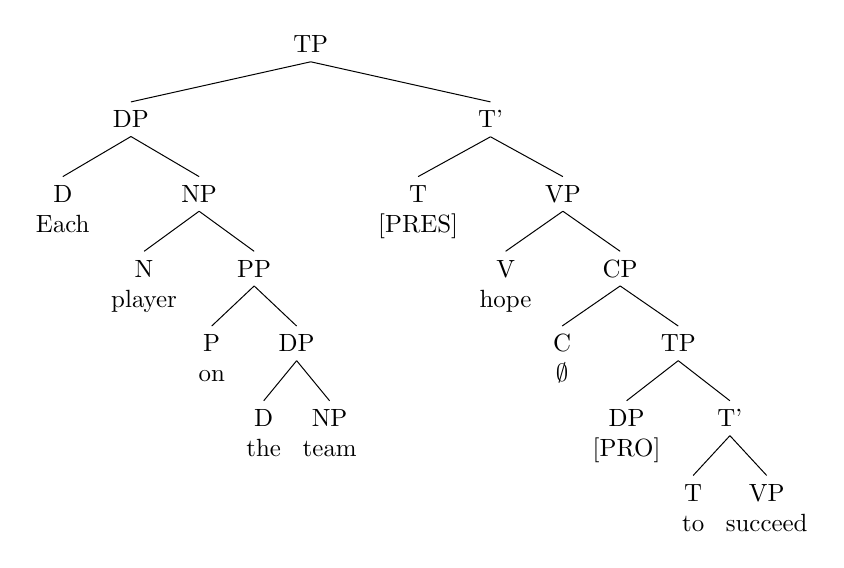
\begin{tikzpicture}[scale=\treeScale, transform shape]
  \tikzset{every tree node/.style={align=center,anchor=north}}
  \Tree [.TP
          [.DP
            D\\Each
            [.NP
              N\\player
              [.PP
                P\\on
                [.DP
                  D\\the
                  NP\\team
                ]
              ]
            ]
          ]
          [.T'
            T\\\feature{PRES}
            [.VP
              V\\hope
              [.CP
                C\\$\emptyset$
                [.TP
                  DP\\\feature{PRO}
                  [.T'
                    T\\to
                    VP\\succeed
                  ]
                ] 
              ]
            ]
          ]
        ]
\end{tikzpicture} \\

\begin{tikzpicture}[scale=\treeScale, transform shape]
  \tikzset{every tree node/.style={align=center,anchor=north}}
  \Tree [.TP
          [.DP
            D\\the
            NP\\children  
          ]
          [.T'
            T\\\feature{PAST}
            [.VP
              [.VP
                V\\deny
                [.DP
                  D\\the
                  NP\\accusation
                ]
              ]
              [.CP
                C\\that
                [.TP
                  DP\\they
                  [.T'
                    T\\had
                    [.VP
                      V\\broken
                      [.DP
                        D\\the
                        NP\\windows
                      ]
                    ]
                  ]
                ]
              ]
            ]
          ]
        ]
\end{tikzpicture} \\

\begin{tikzpicture}[scale=\treeScale, transform shape]
  \tikzset{every tree node/.style={align=center,anchor=north}}
  \Tree [.TP
          [.DP
            D\\\feature{PROP}
            NP\\Yolanda
          ]
          [.T'
            T\\\feature{PAST}
            [.VP
              [.VP
                V\\listen
                [.PP
                  P\\to
                  [.DP
                    [.DP
                      D\\that
                      NP\\woman
                    ]
                    [.D'
                      D\\-s
                      [.NP
                        AP\\detailed
                        NP\\description
                      ]
                    ]
                  ]
                ]
              ]
              [.PP
                P\\of
                [.DP
                  D\\her
                  NP\\misfortunes
                ]
              ]
            ]
          ]
        ]
\end{tikzpicture} \\

\begin{tikzpicture}[scale=\treeScale, transform shape]
  \tikzset{every tree node/.style={align=center,anchor=north}}
  \Tree [.TP
          [.CP
            C\\$\emptyset$
            [.TP
              DP\\\feature{PRO}
              [.T'
                T\\to
                [.VP 
                  V\\locate
                  [.DP
                    D\\the
                    [.NP
                      AP\\lost
                      [.NP
                        N\\contient
                        [.PP 
                          P\\of
                          [.DP 
                            D\\\feature{PROP}
                            NP\\Atlantis
                          ]
                        ]
                      ]
                    ]
                  ]
                ]
              ]
            ]
          ]
          [.T'
            T\\would
            [.VP
              V\\be
              [.DP
                D\\my
                [.NP
                  AP\\greatest
                  NP\\triumph
                ]
              ]
            ]
          ]
        ]
\end{tikzpicture}

\section{Trees in Other Languages}

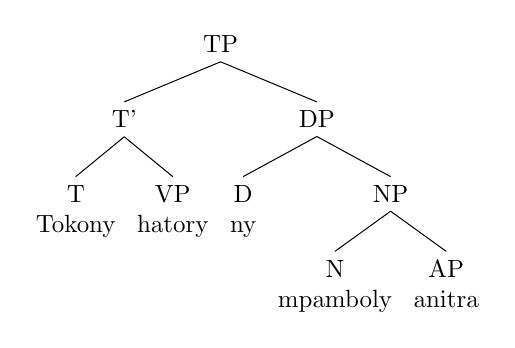
\begin{tikzpicture}[scale=\treeScale, transform shape]
  \tikzset{every tree node/.style={align=center,anchor=north}}
  \Tree [.TP
          [.T'
            T\\Tokony
            VP\\hatory
          ]
          [.DP
            D\\ny
            [.NP
              N\\mpamboly
              AP\\anitra
            ]
          ]
        ]
\end{tikzpicture} \\

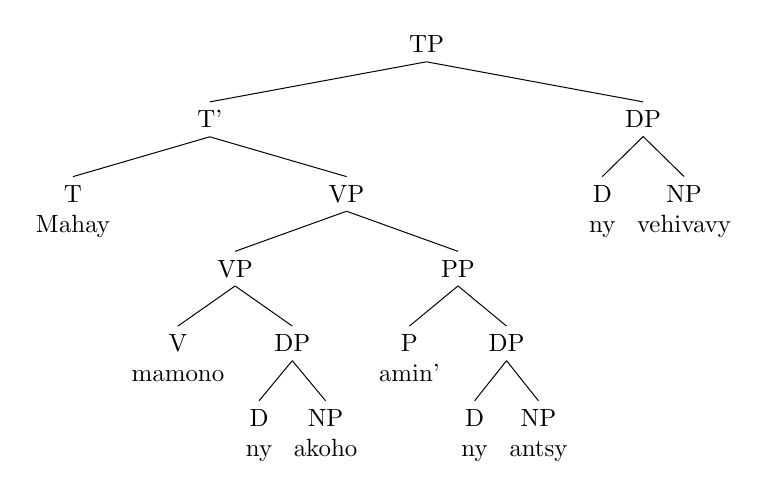
\begin{tikzpicture}[scale=\treeScale, transform shape]
  \tikzset{every tree node/.style={align=center,anchor=north}}
  \Tree [.TP
          [.T'
            T\\Mahay
            [.VP
              [.VP
                V\\mamono
                [.DP
                  D\\ny
                  NP\\akoho
                ]
              ]
              [.PP
                P\\amin'
                [.DP
                  D\\ny
                  NP\\antsy
                ]
              ]
            ]
          ]
          [.DP
            D\\ny
            NP\\vehivavy
          ]
        ]
\end{tikzpicture} \\

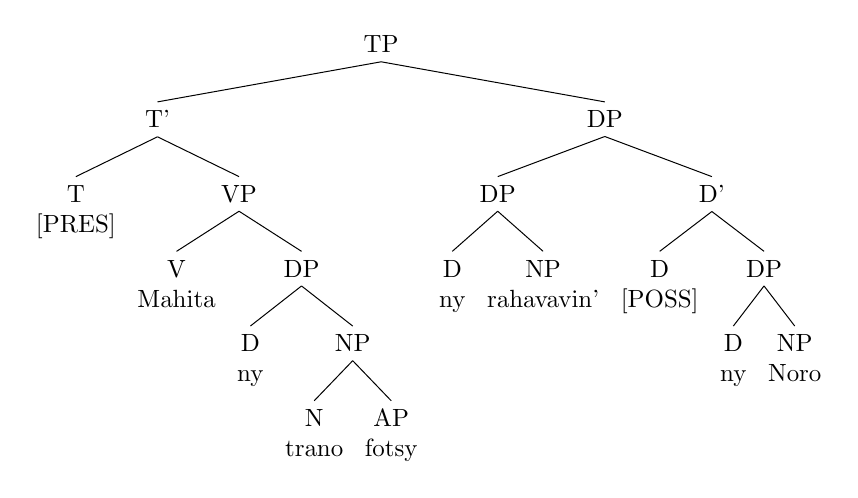
\begin{tikzpicture}[scale=\treeScale, transform shape]
  \tikzset{every tree node/.style={align=center,anchor=north}}
  \Tree [.TP
          [.T'
            T\\\feature{PRES}
            [.VP
              V\\Mahita
              [.DP
                D\\ny
                [.NP
                  N\\trano
                  AP\\fotsy
                ]
              ]
            ]
          ]
          [.DP
            [.DP
              D\\ny
              NP\\rahavavin'
            ]
            [.D'
              D\\\feature{POSS}
              [.DP
                D\\ny
                NP\\Noro
              ]
            ]
          ]
        ]
\end{tikzpicture} \\

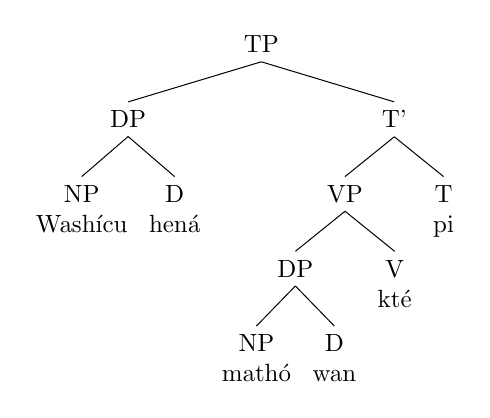
\begin{tikzpicture}[scale=\treeScale, transform shape]
  \tikzset{every tree node/.style={align=center,anchor=north}}
  \Tree
  [.TP
    [.DP
      NP\\Wash\'icu
      D\\hen\'a
    ]
    [.T'
      [.VP
        [.DP
          NP\\math\'o
          D\\wan
        ]
        V\\kt\'e
      ]
      T\\pi
    ]
  ]
\end{tikzpicture} \\

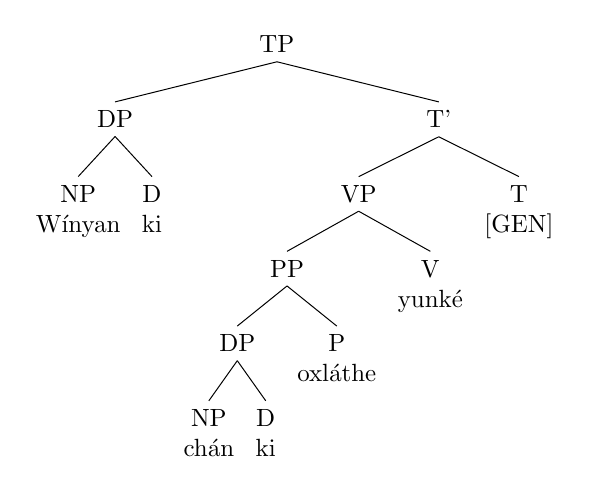
\begin{tikzpicture}[scale=\treeScale, transform shape]
  \tikzset{every tree node/.style={align=center,anchor=north}}
  \Tree
  [.TP
    [.DP
      NP\\W\'inyan
      D\\ki
    ]
    [.T'
      [.VP
        [.PP
          [.DP
            NP\\ch\'an
            D\\ki
          ]
          P\\oxl\'athe
        ]
        V\\yunk\'e
      ]
      T\\\feature{GEN}
    ]
  ]
\end{tikzpicture} \\

In Malagasy the linear ordering of heads and complements is the same as English
but in Lakhota it is reversed. In Lakhota the head appears to always come after
the complement. We only see one reliable instance of a specifier in the
sentences given, the TP structure. Unlike in English, in Malagasy the T' node
comes before the specifier as the auxiliaries appear at the start of the
sentences. With Lakhota I do not think we have enough data to determine if it
differs from English.

\end{document}

